\subsection{Model}

A fluid model of DCQCN was described in~\cite{dcqcn}. The original model
considers N flows with exactly same rates and states, traversing a single
bottleneck link.  In this paper, we extend it to account for flows with
different rates and states.  Instead of having variables that are shared by all
flows, we model each flow individually. The model is shown in
Figure~\ref{fig:dcqcn_model} and Table~\ref{tab:dcqcn_varparam}.

The model assumes that DCQCN is triggered before PFC, and hence ignores the
impact of PFC. Equation~\ref{eq:mark} calculates the probability of a packet
getting marked.  Equation~\ref{eq:q} describes the queue behavior.
Equation~\ref{eq:alpha} captures the evolution of alpha.  Equations~\ref{eq:rt}
and \ref{eq:rc} describe the calculation of target and sending rate,
respectively. 

\begin{figure}[t]
\fbox 
{
\begin{minipage}{\columnwidth}
\begin{equation}
\small
p(t) = \left\{ \begin{array}{ll}
{\rm{0,}} & q(t) \le {K_{\min }}\\
\frac{{q(t) - {K_{\min }}}}{{{K_{\max }} - {K_{\min }}}}{p_{\max }}, & {K_{\min }} < q(t) \le {K_{\max }}\\
{\rm{1,}} & q(t) > {K_{\max }}
\end{array} \right.
\label{eq:mark}
\end{equation}
\begin{equation}
\small
\frac{{dq}}{{dt}} = \sum\limits_{i = 1}^N {R_C^{(i)}(t)}  - C
\label{eq:q}
\end{equation}
\begin{equation}
\small
\frac{{d\alpha^{(i)} }}{{dt}} = \frac{g}{{\tau '}}\left( {\left( {1 - {{(1 - p(t - \tau *))}^{\tau '{R_C}(t - \tau *)}}} \right) - \alpha^{(i)} (t)} \right)
\label{eq:alpha}
\end{equation}
\begin{equation}
\small
\begin{split}
\frac{{d{R_T^{(i)}}}}{{dt}} = & - \frac{{{R_T^{(i)}}(t) - {R_C^{(i)}}(t)}}{\tau }\left( {1 - {{(1 - p(t - \tau *))}^{\tau {R_C^{(i)}}(t - \tau *)}}} \right) \\
& + {R_{AI}}{R_C^{(i)}}(t - \tau *)\frac{{{{(1 - p(t - \tau *))}^{FB}}p(t - \tau *)}}{{{{(1 - p(t - \tau *))}^{ - B}} - 1}} \\
& + {R_{AI}}{R_C^{(i)}}(t - \tau *)\frac{{{{(1 - p(t - \tau *))}^{FT{R_C^{(i)}}(t - \tau *)}}p(t - \tau *)}}{{{{(1 - p(t - \tau *))}^{ - T{R_C^{(i)}}(t - \tau *)}} - 1}}
\end{split}
\label{eq:rt}
\end{equation}
\begin{equation}
\small
\begin{split}
\frac{{d{R_C^{(i)}}}}{{dt}} = & - \frac{{{R_C^{(i)}}(t)\alpha^{(i)} (t)}}{{2\tau }}\left( {1 - {{(1 - p(t - \tau *))}^{\tau {R_C^{(i)}}(t - \tau *)}}} \right) \\
 & + \frac{{{R_T^{(i)}}(t) - {R_C^{(i)}}(t)}}{2}\frac{{{R_C^{(i)}}(t - \tau *)p(t - \tau *)}}{{{{(1 - p(t - \tau *))}^{ - B}} - 1}} \\ 
 & + \frac{{{R_T^{(i)}}(t) - {R_C^{(i)}}(t)}}{2}\frac{{{R_C^{(i)}}(t - \tau *)p(t - \tau *)}}{{{{(1 - p(t - \tau *))}^{ - T{R_C^{(i)}}(t - \tau *)}} - 1}}
\end{split}
\label{eq:rc}
\end{equation}
\end{minipage}
}
\caption{DCQCN fluid model}
\label{fig:dcqcn_model}
\end{figure}
\begin{table}
\center
{
\footnotesize
{
\begin{tabular}{|c|c|}
\multicolumn{2}{l}{\bf Variables} \\ \hline
$R_c$ & Current Rate \\ \hline
$R_t$ & Target Rate \\ \hline
$\alpha$ & See Equation (\ref{eq:rp_dec}) \\ \hline
$q$ & Queue Size \\ \hline
$t$ & Time \\ \hline
\multicolumn{2}{c}{} \\
\multicolumn{2}{l}{\bf Parameters} \\ \hline
$K_{min}, K_{max}, P_{max}$ & RED marking parameters. \\ \hline
$g$ & See Equation (\ref{eq:rp_dec}) \\ \hline
$N$ & Number of flows at bottleneck\\ \hline
$C$ & Bandwidth of bottleneck link\\ \hline
$F$ & Fast recovery steps (fixed at 5) \\ \hline
$B$ & Byte counter for rate increase\\ \hline
$T$ & Timer for rate increase\\ \hline
$R_{AI}$ & Rate increase step (fixed at 40Mbps)\\ \hline
$\tau *$ & Control loop delay \\ \hline
$\tau '$ & Interval of Equation (\ref{eq:rp_alpha_recover})\\ \hline
\end{tabular}
}
}
\caption{DCQCN Fluid model variables and parameters}
\label{tab:dcqcn_varparam}
\end{table}

\para{Model Validation:}
In~\cite{dcqcn} it was shown that the fluid model shown in
Figure~\ref{fig:dcqcn_model} matches actual hardware implementation. Here we
only show our NS3 packet-level simulations are in agreement with the model.We
model a simple topology, in which N senders, connected to a switch, send to a
single receiver, also connected to that switch. DCQCN parameters are set to the
values proposed in~\cite{dcqcn}. Note that as per DCQCN specification, all flows
start at line rate. In Figure~\ref{fig:dcqcn_validation} we compare rate of one
of the N flows, for both fluid model and the NS3 simulations. We see the fluid
model and the simulator are in good agreement, and unsurprisingly, the agreement
gets better as N increases.

\begin{figure*}[t]
\center
\subfigure[N=2] { 
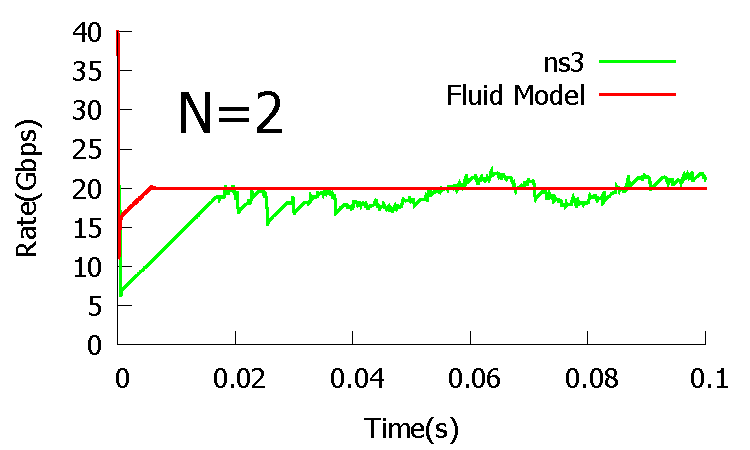
\includegraphics[width=0.3\textwidth]{figures/dcqcn_validation_2_rate.pdf}
}
\subfigure[N=10] { 
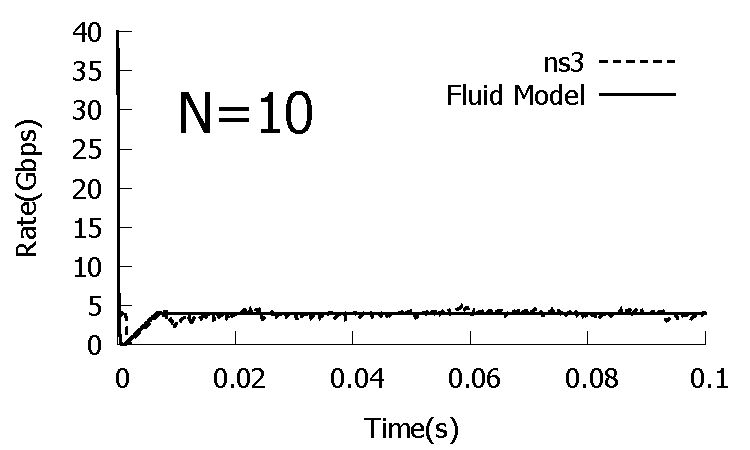
\includegraphics[width=0.3\textwidth]{figures/dcqcn_validation_10_rate.pdf}
}
\subfigure[N=20] { 
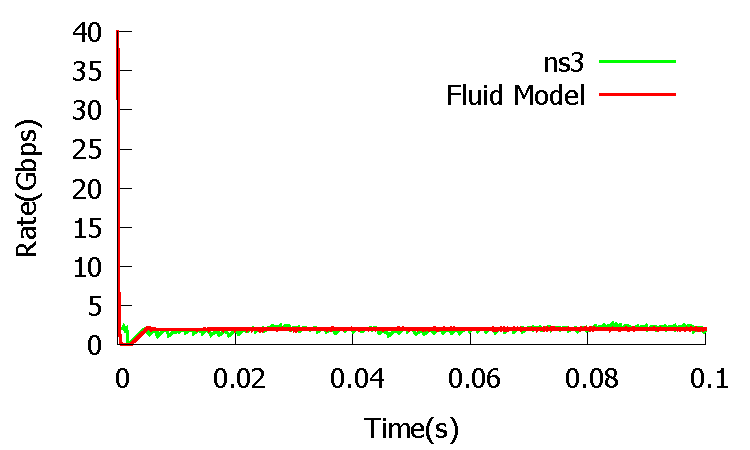
\includegraphics[width=0.3\textwidth]{figures/dcqcn_validation_20_rate.pdf}
}
\caption{Comparison of DCQCN fluid model and NS3 simulations}
\label{fig:dcqcn_validation}
\end{figure*}
